\chapter{Temperature, and other species}\label{ch:temperature}

\section{The floor is a function of temperature}

The Mahaffey number falls as body temperature rises, if the free energy of ATP hydrolysis is held fixed: 22.94 for a salmonid
at 10~\textdegree C, 20.94 for a human at 37~\textdegree C, 20.84 for a dog at 38.5~\textdegree C, 20.74 for a bird at
40~\textdegree C. \calc{} Holding $\dGATP$ fixed is an assumption; the free energy depends on temperature and on the cell's
ATP, ADP and phosphate concentrations.

The floor of Eq.~\eqref{eq:eps0} makes a sharper statement. If a cell holds each site with a fixed energy $E_{\rm hold}$,
measured at 37~\textdegree C as $3.41\,\kB T$, then at another temperature
\begin{equation}
  \varepsilon_0(T)=\frac{1}{1+\exp\!\left(E_{\rm hold}/\kB T\right)} ,
  \label{eq:eps0T}
\end{equation}
with no exponent to choose. \derived{} given a fixed holding energy. At 10~\textdegree C this gives $\varepsilon_0=0.0233$ and a
floor $0.78$ times the human one; at 38.5~\textdegree C, $1.012$ times (Figure~\ref{fig:eps0T}). \calc{} The alternative is a
cell that holds its error fixed in units of $\kB T$, adjusting its holding energy with temperature. The two are distinguished by
one measurement.

\begin{figure}[htbp]\centering
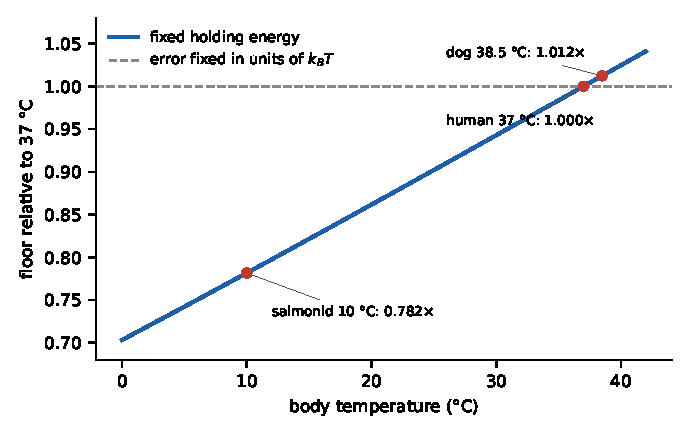
\includegraphics[width=0.8\textwidth]{figures/part6/fig_eps0_T.pdf}
\caption{The floor against body temperature. Solid: fixed holding energy ($3.41\,\kB T$ at 37~\textdegree C), Eq.~\eqref{eq:eps0T}.
Dashed: error held fixed in units of $\kB T$. Marks: dog (38.5~\textdegree C), human (37~\textdegree C), salmonid
(10~\textdegree C). \calc}
\label{fig:eps0T}
\end{figure}

\paragraph{Birds, reptiles, and the enzyme itself.} Birds present a complementary test: at 39--42~\textdegree C, warmer than
most mammals, a fixed holding energy puts their floor $1.025$ times the human one at 40~\textdegree C and $1.041$ times at
42~\textdegree C; reptiles at 25--32~\textdegree C sit at $0.902$--$0.959$ times, and a cell at 15~\textdegree C at
$0.821$ times. \calc{} The same prediction can be made without any animal. DNMT1 maintenance fidelity should be
measurable as a function of temperature in controlled in vitro experiments, from 15~\textdegree C to 42~\textdegree C,
spanning the full vertebrate range. If the enzyme discriminates hemimethylated from unmethylated sites by a fixed energy, a
preference $S$ measured at 37~\textdegree C becomes $S^{310.15\,\mathrm{K}/T}$ at temperature $T$: the published 7-fold rises
to 8.1 at 15~\textdegree C and falls to 6.8 at 42~\textdegree C, and 80-fold becomes 112 and 75. \calc{} If instead the
preference is the same at every temperature, the enzyme holds its error fixed in units of $\kB T$ (the dashed line of
Figure~\ref{fig:eps0T}). This is measurable by single-molecule DNMT1 kinetics --- a direct test in a cell-free system.
\prediction

\section{Reading ectotherms}

The test is one species, one cell type and one pipeline at two recorded temperatures, each fish read against its own floor on single
molecules, with molecular identifiers and a known-pattern control in every library so that the library's own errors are read and removed.
The floor at 10~\textdegree C is measured on fish, not assumed. \prediction{} The salmonid sets read in development are in the
development log (\href{https://github.com/hmahaffeyges/IAM-Validation/tree/main/development}{\texttt{development/}}).

\paragraph{Published values for ectotherms are a different quantity.} The global methylation values published for reptiles,
amphibians and fish come from reversed-phase high-performance liquid chromatography of hydrolysed
DNA~\cite{Varriale2006_fish,Varriale2006_reptile}. This technique measures the total 5mC/C ratio across the entire genome,
including repetitive elements, transposable elements and intergenic regions. \observed{} It is a different quantity from
a per-site $\beta$ on the sites that make a cell what it is, and from the mean of per-site entropies that the gauge reads, so
no such value is placed on the gauge. \derived{} (from the definitions, Chapter~\ref{ch:surface}) The definitive route
is to read ectotherm cells with a site-resolved method on one pipeline --- an array with degenerate probes designed to
tolerate cross-species sequence variation~\cite{Arneson2022}, or read-level single-molecule sequencing.


\begin{keybox}[title=The test that decides]
One species, one cell type, one read pipeline, at two recorded temperatures. A rearing-temperature experiment does it; a
public whole-genome coho data set (BioProject PRJNA641939), downloaded and not yet read, would give the first fish reading on a pipeline comparable to the human one. Until then
the temperature behaviour of the floor is \openprob, and no ectotherm is read on the gauge.
\end{keybox}

\section{Other species}\label{sec:p4_species}

Why do mammals live so differently? The house mouse and the human share most of their genes: about 80~\% of mouse genes
have a single identifiable orthologue in the human genome~\cite{Waterston2002}. Their cellular machinery is nearly identical
at the molecular level. Yet a house mouse lives four years and a bowhead whale two centuries~\cite{Tacutu2018}. \observed

Epigenetic clocks have documented a deep connection between DNA methylation and lifespan. Lowe and co-workers showed that the
\emph{rate} of methylation change at age-associated CpG sites falls with maximum lifespan across six mammalian
species~\cite{Lowe2018}, and Crofts and co-workers found the same scaling at conserved age-related sites across 42
species~\cite{Crofts2024}. Universal pan-mammalian clocks built on 11,754 arrays from 185 species estimate age with
$r>0.96$~\cite{Lu2023}, and the co-methylation networks underlying mammalian traits have been mapped across 15,456 profiles
from 348 species~\cite{Haghani2023}. The empirical pattern is robust: methylation tracks lifespan. \observed{}

What has been missing is a \emph{physical explanation} for why this is so. These clocks are statistical: trained regression
models that identify CpGs correlated with age. They accurately describe what happens. They do not derive from first
principles why it happens. \interp{}
The gauge of this Part does not answer that question either; what it adds is a floor with a temperature in it,
Eq.~\eqref{eq:eps0T}, so that a cell of any species can in principle be read against the same physics once its own healthy
cells have been referenced.

\section{Dogs}

Dogs are the natural first mammal after humans: their blood is drawn routinely, they share our environment, and a
methylation array designed for mammals covers conserved CpGs across species~\cite{Arneson2022}. For a dog $M=20.84$ and the
floor moves by about 1~\%. The first step is a canine healthy reference from purified canine blood cells; then sorted healthy
canine cells read on it, held out, should land at 1.00. \prediction

\section{Where the gauge can apply}

The gauge applies wherever DNMT1-mediated CpG maintenance methylation is the primary mechanism of epigenomic identity
preservation, because what it reads is the error of that copy. This criterion is satisfied in the jawed vertebrates ---
mammals, birds, reptiles, amphibians and fish --- where DNMT1 is the conserved maintenance methyltransferase~\cite{Lyko2018}.
\observed{} The gauge does \emph{not} directly apply to \emph{Drosophila}, which has no DNMT1 and at most trace cytosine
methylation, nor to \emph{C.~elegans}, where cytosine methylation is absent~\cite{Lyko2018}; insects with gene-body
methylation only, such as the honey bee, carry DNMT1 but its function differs from vertebrate maintenance~\cite{Lyko2010}.
\observed{} Corals and sea anemones are the open case: they carry DNMT1 and live for decades, but whether their methylation
maintains identity or regulates genes is not known, and no floor is proposed for them. \openprob{} The scope is itself a
statement about the instrument: a floor read from a copy error exists only where a copy is made. \interp
